\documentclass[tikz,border=5pt]{standalone}

\usetikzlibrary{calc, intersections}
\usepackage{xfp}
\usepackage{mathrsfs} % Añade el macro \mathscr que usamos para nombrar circunferencias: \mathscr{C_1}

\begin{document}
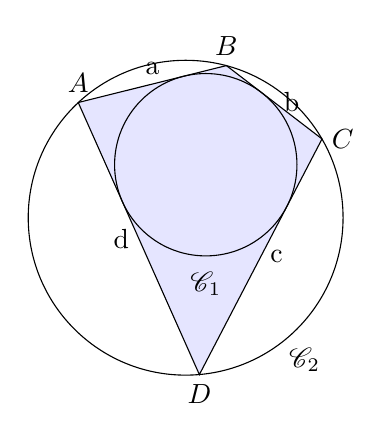
\begin{tikzpicture}

\def\R{2}

% Un cuadrado es un cuadrilátero bicéntrico.
\def\angleA{45}
\def\angleB{135}
\def\angleC{225}
\def\angleD{315}

% Otro cuadrilátero bicéntrico
\def\angleA{133}
\def\angleB{75}
\def\angleC{30}
\def\angleD{275}

% Otro cuadrilátero bicéntrico
%% \def\angleA{0}
%% \def\angleB{45}
%% \def\angleC{160}
%% \def\angleD{302}

% Otro cuadrilátero bicéntrico
%% \def\angleA{0}
%% \def\angleB{58}
%% \def\angleC{103}
%% \def\angleD{218}

% Otro cuadrilátero bicéntrico
%% \def\angleA{0}
%% \def\angleB{142}
%% \def\angleC{257}
%% \def\angleD{302}

\coordinate (A) at ({\R*cos(\angleA)}, {\R*sin(\angleA)});
\coordinate (B) at ({\R*cos(\angleB)}, {\R*sin(\angleB)});
\coordinate (C) at ({\R*cos(\angleC)}, {\R*sin(\angleC)});
\coordinate (D) at ({\R*cos(\angleD)}, {\R*sin(\angleD)});

% We use overlay to make standalone omit these segments when
% computing the dimensions of the final PDF.
\path let \p1=(A), \p2=(B), \p3=(C), \p4=(D) in node[overlay] {
    % Calculate 4 sides
    \xdef\sideAB{\fpeval{sqrt((\x2-\x1)^2 + (\y2-\y1)^2)}}
    \xdef\sideBC{\fpeval{sqrt((\x3-\x2)^2 + (\y3-\y2)^2)}}
    \xdef\sideCD{\fpeval{sqrt((\x4-\x3)^2 + (\y4-\y3)^2)}}
    \xdef\sideDA{\fpeval{sqrt((\x1-\x4)^2 + (\y1-\y4)^2)}}
    % Calculate 2 diagonals
    \xdef\diagonalAC{\fpeval{sqrt((\x3-\x1)^2 + (\y3-\y1)^2)}}
    \xdef\diagonalBD{\fpeval{sqrt((\x4-\x2)^2 + (\y4-\y2)^2)}}
};

\edef\isTangentialNumber{\fpeval{abs((\sideAB + \sideCD) - (\sideBC + \sideDA))}}
\edef\isTangentialBoolean{\fpeval{\isTangentialNumber < 0.001 ? 1 : 0}}
\edef\isCyclicNumber{\fpeval{abs(\diagonalAC*\diagonalBD - (\sideAB*\sideCD + \sideBC*\sideDA))}}
\edef\isCyclicBoolean{\fpeval{\isCyclicNumber < 0.001 ? 1 : 0}}

\ifnum\isTangentialBoolean=1
   \ifnum\isCyclicBoolean=1

        %% Draw quadrilateral and labels

        \draw[fill=blue!10!white]
                 (A) node[above]{$A$}
              -- node [above]{a} (B) node[above]{$B$}
              -- node [right]{b} (C) node[right]{$C$}
              -- node [right]{c} (D) node[below]{$D$}
              -- node [left]{d} cycle;

        %% Draw incircle

        \coordinate(G1) at ($(A)!1cm!(B)$);
        \coordinate(G2) at ($(A)!1cm!(D)$);
        \coordinate(M1) at ($(G1)!.5!(G2)$);
        \path[name path=angleBisector1]
            let \p1=(A), \p2=(C), \n1={veclen(\y2-\y1,\x2-\x1)}
            in (A) -- ($(A)!\n1!(M1)$);

        \coordinate(H1) at ($(B)!1cm!(A)$);
        \coordinate(H2) at ($(B)!1cm!(C)$);
        \coordinate(M2) at ($(H1)!.5!(H2)$);
        \path[name path=angleBisector2]
            let \p1=(B), \p2=(D), \n1={veclen(\y2-\y1,\x2-\x1)}
            in (B) -- ($(B)!\n1!(M2)$);

        \draw [name intersections={of=angleBisector1 and angleBisector2, by={centerOfIncircle}}]
            let \p1=(centerOfIncircle), \p2=($(A)!(centerOfIncircle)!(B)$), \n1={veclen(\y2-\y1,\x2-\x1)}
            in (centerOfIncircle) circle [red, radius=\n1]
            \pgfextra{\xdef\radiusOfIncircle{\n1}};

        %% Draw circumcircle

        \coordinate (M1) at ($(A)!0.5!(B)$);
        \path[name path=bisectorAB, overlay] ($(M1)!10!-90:(B)$) -- ($(M1)!10!90:(B)$);

        \coordinate (M2) at ($(B)!0.5!(C)$);
        \path[name path=bisectorBC, overlay] ($(M2)!10!90:(C)$) -- ($(M2)!10!-90:(C)$);

        \draw [name intersections={of=bisectorAB and bisectorBC, by={centerOfCircumcircle}}]
            let \p1=(centerOfCircumcircle), \p2=(A), \n1={veclen(\y2-\y1,\x2-\x1)}
            in (centerOfCircumcircle) circle [radius=\n1]
           \pgfextra{\xdef\radiusOfCircumcircle{\n1}};

        % Show labels for incircle and circumcircle
        \def\offset{10}
        \def\incircleAngleLabel{270}
        \draw node at ($(centerOfIncircle) + (\incircleAngleLabel:\radiusOfIncircle + \offset)$) {$\mathscr{C}_1$};
        \def\circumcircleAngleLabel{310}
        \draw node at ($(centerOfCircumcircle) + (\circumcircleAngleLabel:\radiusOfCircumcircle + \offset)$) {$\mathscr{C}_2$};
    \else
        \node[red, font=\bfseries] at (0,0) {This quadrilateral is tangential, but is not cyclic. \isCyclicNumber};
    \fi
\else
    \node[red, font=\bfseries] at (0,0) {This quadrilateral is not tangential. \isTangentialNumber};
\fi


\end{tikzpicture}
\end{document}
